\paragraph\
In this chapter we have tested scalability of \emph{ntop} with RRDTool, \emph{ntop} with cassandra and  Open vSwitch with Cassandra. We have used 32KB, 64KB, 128KB socket buffer for \emph{ntop} and SWSR IPC buffer for Open vSwitch to test behavior of our solutions. Using \emph{netperf} \cite{netperf} tool we have generated traffic. 

\paragraph\
In the first section we present \emph{netperf} tool. In Section \ref{testbed}, we present our test environment. We have presented results and
discussion in the Section \ref{result_and_Dis}. Finally we conclude with Section \ref{Result_conclusion}.

\section{\emph{netperf}} \label{etperf}
\paragraph\
	\emph{netperf} is a benchmark tool that can be use to measure various aspect of networking performance. The primary focus are bulk  data transfer and request/response performance using either TCP or UDP and the Berkeley Sockets interface. Using \emph{netperf} we can perform following 
	tests \cite{netperf}
	\begin{enumerate}
	 \item TCP and UDP unidirectional transfer and request/response over IPv4 and IPv6 using the Sockets interface. 
	 \item TCP and UDP unidirectional transfer and request/response over IPv4 using the XTI interface. 
	 \item Link-level unidirectional transfer and request/response using the DLPI interface. 
	 \item Unix domain sockets.
	 \item SCTP unidirectional transfer and request/response over IPv4 and IPv6 using the sockets interface. 
	\end{enumerate}
\paragraph\
	TCP Connect/Request/Response measures the performance of establishing a connection, exchanging a single request/response transaction, and tearing-down that connection. TCP\_CRR creates two new flow for every request/response transaction. In a TCP\_CRR performance test, a \emph{netperf} 	creates lots of flow which can be monitored by Open vSwitch or any other NetFlow enabled router/switch. Using TCP\_CRR we simulate a heavy loaded network in our lab. In the next section we present our testbed that uses \emph{netperf} for generating NetFlow packets for our tests. 

\section{Test Environment Setup} \label{testbed}
	Our test environment contains multiple components as described in the Table \ref{table_testbed}. We have use KVM, Open vSwitch to create virtual network that generates NetFlow packets using Open vSwitch. Figure \ref{figure_testbed} illustrate our experimental testbed. Each of our system Sys-1, 2, 3, 4 are running OpenSuse-12.2(Linux 3.4 kernel). Sys-1 and 2 are using latest version of KVM. Sys-1 and 2 have 5 virtual machines each of them running 25 \emph{netperf} clients.% Ma'am I'm not able form the next sentense properly
	one VM each from both Sys-1 and Sys-2 forms five pairs of VM. Each pairs of VM have 25 \emph{netperf} clients each sending traffic to each other. With 25 \emph{netperf} running on both Sys-1 and Sys-2, we get approximately 1000 NetFlow packets/second. Figure \ref{peakNetperf} illustrates out claim. So all together the testbed runs 250 \emph{netperf} clients. In the next section we describe about our tests that we have done using this testbed.
	\begin{table}
	\centering
	 \begin{tabular}{|l|l|}
	  \hline
	  \textbf{Component Name} & \textbf{Details/Version} \\ \hline
	  CPU   & Intel(R) Core(TM) i5-2400 CPU @ 3.10GHz. \\ \hline
	  Operating System & OpenSuse 12.2 \\ \hline
	  Linux Kernel & 3.4 \\ \hline
	  KVM          & kvm-1.1.1-1.8.1 \\ \hline
	  Open vSwitch & openvswitch-1.9.0(LTS) \\ \hline
	  \emph{netperf} & netperf-2.6 \\ \hline
	  \emph{ntop}    & ntop-5.0.1 \\ \hline
	  Cassandra      & Apache-cassndra-1.2.5 \\ \hline	  
	 \end{tabular}
	  \label{table_testbed}
	  \caption{Components of Our Testbed}
	\end{table}

	\begin{figure}[htb]
	  \centering
	  \includegraphics[scale=.3]{testbed}
	  \caption{Evaluation Testbed } 
	  \label{figure_testbed}
	\end{figure}
	\begin{figure}[htb]
	  \centering
	  \includegraphics[scale=1]{data/peaknetperf}
	  \caption{NetFlow Packet generated with \emph{netperf}} 
	  \label{peakNetperf}
	\end{figure}
	
\section{Analysis and Discussion of Test Results} \label{result_and_Dis}
\paragraph\
	We have tested scalability of the following conditions with various socket buffer SWSR IPC buffer sizes. 
	\begin{enumerate}
	 \item \emph{ntop} and RRDTool.
	 \item \emph{ntop} storing NetFlow records to Cassandra.
	 \item Open vSwitch storing into NetFlow records directly into Cassandra.
	\end{enumerate}
	\paragraph{\emph{ntop} and RRDTool:} In this test, we have generated NetFlow packets with Sys-1 and Sys-2 and Open vSwitch 
	of Sys-2 exports NetFlow packets to \emph{ntop} running on Sys-3. \emph{ntop} uses RRDTool to analysis and store NetFlow
	statistics.
	\paragraph{\emph{ntop} and Cassandra:} In this test, we have run the similar test excepts Cassandra us used to store NetFlow records.
	\paragraph{Open vSwitch and Cassandra:} In this test, Open vSwitch stores NetFlow records directly using NfCassaStore as described in pervious chapter.
	 
	\subsection{Analysis of the Graphs}
	\paragraph\
		Figure \ref{graph32}, \ref{graph64} and \ref{graph128} illustrate about number of packet drops in all three test cases with buffer size 32KB, 64KB and 128KB. Number of drops with RRDTool is very less with respect to other two.
		Open vSwitch with Cassandra tests improves better than \emph{ntop} storing into Cassandra if we increase amount of buffer. 
	\begin{figure}[!htb]
	    \centering
	    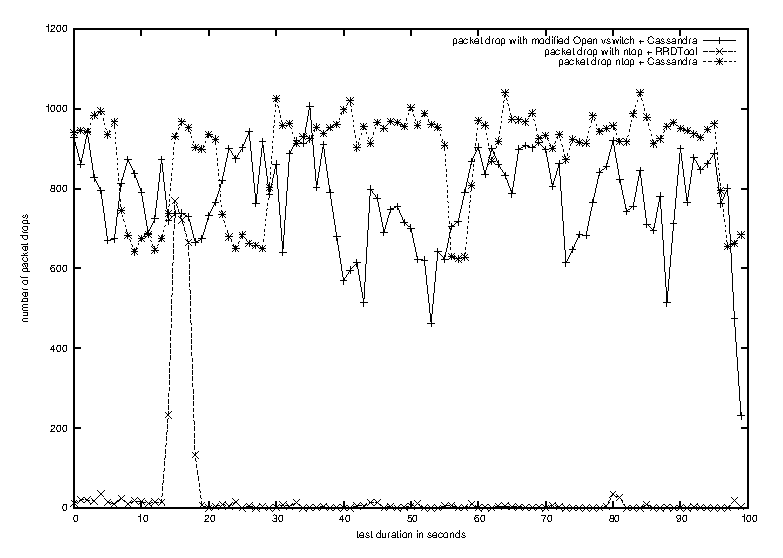
\includegraphics[scale=1]{data/out32}
	    \caption{Packet Drops with 32 KB Socket and IPC buffer size} 
	    \label{graph32}
	  \end{figure}
	
	  \begin{figure}[!htb]
	    \centering
	    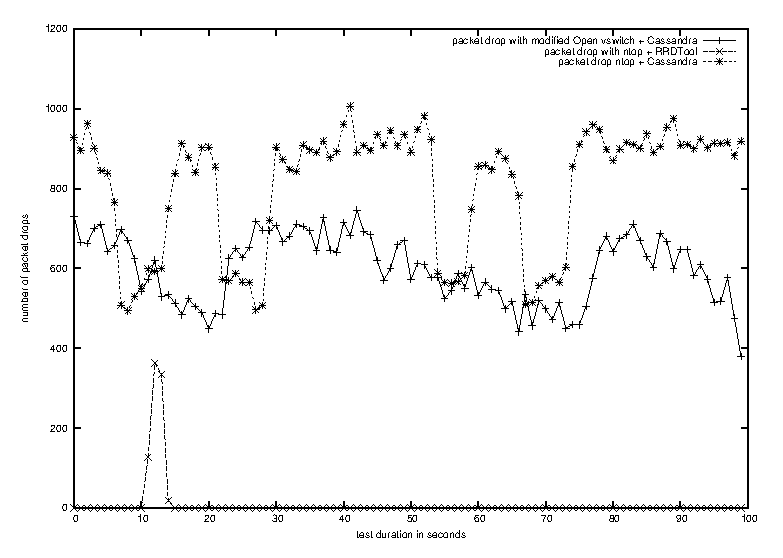
\includegraphics[scale=1]{data/out64}
	    \caption{Packet Drops with 64 KB Socket and IPC buffer size } 
	  \label{graph64}
	  \end{figure}
	  
	  \begin{figure}[!htb]
	    \centering
	    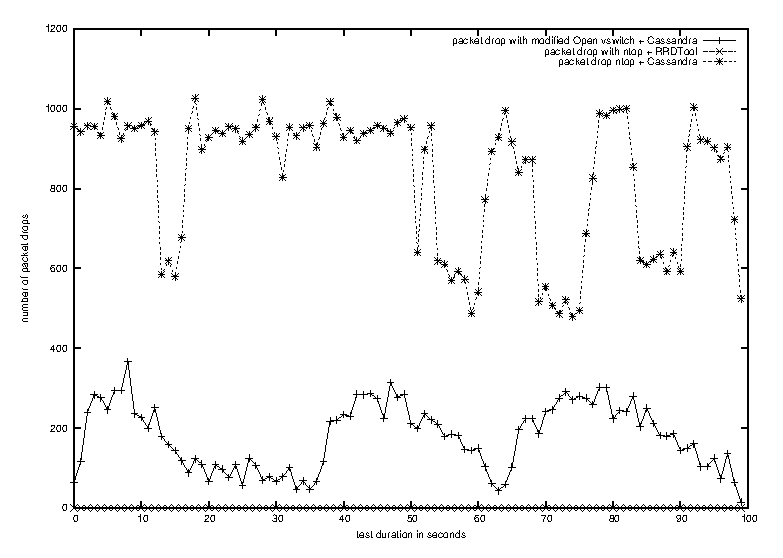
\includegraphics[scale=1]{data/out128}
	    \caption{Packet Drops with 128 KB Socket and IPC buffer size} 
	    \label{graph128}
	  \end{figure}
	  If we look at the detail operations that take place during our three tests, we may get more insights to analyze the results.
	  Operations done by \emph{ntop} with RRDTool:
	  \begin{enumerate}
	   \item Read NetFlow Packets from socket.
	   \item Analysis NetFlow packets 
	   \item Store NetFlow statistics into RRD with disk write.
	  \end{enumerate}
	  \emph{ntop} with Cassandra does similar operations except it stores NetFlow records into Cassandra using our Cassandra C client.
	  On the other hand Open vSwitch use \emph{Pycassa} to store NetFlow records into Cassandra. In both case, \emph{ntop} with RRDTool and Open vSwitch with Cassandra, a NetFlow packet pass thorugh network once and then stored into disk. In \emph{ntop} with Cassandra test, a Netflow packet has to pass through network twice, that explains why \emph{ntop} with Cassandra drops more packets than other two. \emph{ntop} with RRDTool is faster because RRDTool is written in c and dynamically linked with \emph{ntop}. Open vSwitch use Python, which is interpreted language and slower than
	  C.
	  \emph{ntop} with Cassandra does not improve its performance much with compare with Open vSwitch even we increase Socket buffer size.
	  \emph{ntop} uses our own Cassandra C client for storing data into Cassandra. Cassandra C client has pass through multiple layers of API calls (C-Python API, $Pycassa$ API, thrift API)	before reaching to Cassandra which is one reason for bad performance of \emph{ntop} with Cassandra. 
	  \paragraph\
	  
	  
	  

	  
\section{Conclusion} \label{Result_conclusion}